\documentclass[../main.tex]{subfiles}

\begin{document}
	
Siguiendo la línea trazada en el capítulo anterior, en el presente exploraremos el siguiente nivel en la jerarquía de Chomsky, las gramáticas de tipo II o gramáticas libres de contexto. \\
Los lenguajes regulares, a pesar de su gran utilidad, su restricción a patrones simples los vuelve muy limitados y poco adecuados para la descripción del lenguaje natural. Siguiendo el ejemplo en \cite{Kulacka2012}, un lenguaje de la forma $\{ a^i b c^i|i \in \mathbb{N} \}$ no es regular\footnote{Esta es una consecuencia inmediata del lema del bombeo para lenguajes regulares cuyo enunciado y prueba puede consultarse en \cite{hopcroft01}} y corresponde a la anidación de elementos, así oraciones del tipo ''Si el pasto es verde, entonces el pasto es verde'', ''Si si el pasto es verde, entonces el pasto es verde, entonces el pasto es verde'' que se describen con la gramática $\{ (\text{Si})^i \text{ el pasto es verde, } (\text{entonces el pasto es verde})^i | i \in \mathbb{N}\}$ no serían gramaticalmente válidas en el español, pero lo son (a pesar de su
poca naturalidad). \\
Por ello, surge  el estudio de los lenguajes libres de contexto, clásicamente definidos mediante gramáticas de nombre homónimo, árboles de derivación o por medio de autómatas con pila \textemdash autómatas que tienen memoria \textemdash. \\
Por la vía categórica, en este capítulo mostraremos que gramáticas definidas mediante multicategorías, categorías donde los morfismos tienen como dominio más de un objeto, tienen exactamente el mismo poder expresivo que los lenguajes libres de contexto. 

\section{Multicategorías}

Como en el capítulo anterior, comenzaremos dando los ingredientes para describir una multicategoría libre. 

\begin{dfn}
	Una \textbf{signatura de multicategoría} $H$ es un conjunto de nodos $H_1$ y uno de objetos \(H_0\) junto a un par de funciones
	\[
		H_0^* \xleftarrow{\dom} H_1 \xrightarrow{\cod} H_0
	\] 
	Un morfismo de signaturas de multicategorías $\varphi : H \to \Gamma$ es un par de funciones $\varphi_0 : H_0 \to \Gamma_0$ y $\varphi_1 : H_1 \to \Gamma_1$ tales que el siguiente diagrama conmuta: 
	\[
	\begin{tikzcd}
		H_0^* \arrow{d}{\phi_0} & H_1 \arrow{r}{\tt{dom}} \arrow{l}{\tt{cod}} \arrow{d}{\phi_1} & H_1 \arrow{d}{\phi_0} \\
		\Gamma_0^* & \Gamma_1 \arrow{r}{\tt{dom}} \arrow{l}{\tt{cod}} & \Gamma_1
	\end{tikzcd}
	\]
	Con tales morfismos, las signaturas de multicategorías forman la categoría \textbf{MultiSig}.
\end{dfn}
\noindent Dado una signatura de multicategoría, denotaremos un nodo $b_1...b_n \xrightarrow{f} a$ gráficamente como: 
	
	\begin{center}
	\begin{tikzpicture}[node distance={10mm}, thick, main/.style = {draw, circle, fill=black, inner sep=0pt, minimum width=2pt},
		letter/.style={circle,draw=white,very thick}] 
		
		\node[main] (1) {};
		\node[letter] (2) [right of=1] {$\cdots$};
		\node[main] (3) [right of=2]{};
		\node[main] (4) [below of=2]{};
		\node[main] (5) [below of=4]{};
		
		\draw[-] (1) -- (4);
		\draw[-] (3) -- (4);
		\draw[-] (4) -- (5);
		
		\node[letter] (p) at (-0.5,0) {$b_1$};
		\node[letter] (p) at (2.5,0) {$b_n$};
		\node[letter] (p) at (1.5,-1) {$f$};
		\node[letter] (p) at (1.5,-2) {$a$};
	\end{tikzpicture}
	\end{center}
Además, diremos que $f$ tiene aridad $n$.

\begin{ej}
	\label{ej:RealSig}
	Consideremos la siguiente signatura de multicategoría donde los objetos corresponderán a los números reales, $\mathbb{R}$. Luego, dado $a, ab \in \mathbb{R}^*$ tenemos los siguientes nodos: 
	\begin{multicols}{4}
			\begin{center}
			\begin{tikzpicture}[node distance={10mm}, thick, main/.style = {draw, circle, fill=black, inner sep=0pt, minimum width=2pt},
				letter/.style={circle,draw=white,very thick}] 
				
				\node[main] (1) {};
				\node[main] (4) (p) at (0,-2){};
				
				\draw[-] (1) to (0,-2);
				
				\node[letter] (p) at (-0.5,0) {$a$};
				\node[letter] (p) at (-0.5,-2) {$a$};
			\end{tikzpicture}
		\end{center}
		
			\begin{center}
				\begin{tikzpicture}[node distance={10mm}, thick, main/.style = {draw, circle, fill=black, inner sep=0pt, minimum width=2pt},
					letter/.style={circle,draw=white,very thick}] 
					
					\node[main] (1) {};
					\node[main] (4) (p) at (0,-2){};
					
					\draw[-] (1) to (0,-2);
					
					\node[letter] (p) at (-0.5,0) {$a$};
					\node[letter] (p) at (-0.5,-2) {$-a$};
				\end{tikzpicture}
			\end{center}
		
			\begin{center}
			\begin{tikzpicture}[node distance={10mm}, thick, main/.style = {draw, circle, fill=black, inner sep=0pt, minimum width=2pt},
				letter/.style={circle,draw=white,very thick}] 
				
				\node[main] (1) {};
				\node[main] (2) (p) at (1.5, 0) {};
				\node[main] (3) (p) at (.75, -1) {};
				\node[main] (4) (p) at (.75, -2) {};

				
				\draw[-] (1) to (.75, -1);
				\draw[-] (1.5, 0) to (.75, -1);
				\draw[-] (.75,-1) to (.75, -2);
				
				\node[letter] (p) at (-.5,0) {$a$};
				\node[letter] (p) at (2,0) {$b$};
				\node[letter] (p) at (1.35,-2) {$a+b$};
				
			\end{tikzpicture}
			\end{center}
		
			\begin{center}
				\begin{tikzpicture}[node distance={10mm}, thick, main/.style = {draw, circle, fill=black, inner sep=0pt, minimum width=2pt},
					letter/.style={circle,draw=white,very thick}] 
					
					\node[main] (1) {};
					\node[main] (2) (p) at (1.5, 0) {};
					\node[main] (3) (p) at (.75, -1) {};
					\node[main] (4) (p) at (.75, -2) {};
					
					
					\draw[-] (1) to (.75, -1);
					\draw[-] (1.5, 0) to (.75, -1);
					\draw[-] (.75,-1) to (.75, -2);
					
					\node[letter] (p) at (-.5,0) {$a$};
					\node[letter] (p) at (2,0) {$b$};
					\node[letter] (p) at (1.35,-2) {$a\cdot b$};
					
				\end{tikzpicture}
			\end{center}
	\end{multicols}
	\noindent Notemos que los primeros dos nodos corresponden a las operaciones de aridad $1$ que lleva un número asímismo o a su inverso aditivo respectivamente. Por otro lado, los últimos dos nodos corresponden a las operaciones binarias usuales de los números reales: la adición y la multiplicación. \\
	Notemos, además, que para cualquier $abc \in \mathbb{R}^*$ tenemos que, dado que nuestras operaciones son asociativas, entonces $a+(b+c)=(a+b)+c$, así gráficamente tenemos la igualdad de los siguientes diagramas:
	
	\begin{center}
	\begin{tikzpicture}[node distance={10mm}, thick, main/.style = {draw, circle, fill=black, inner sep=0pt, minimum width=2pt},
		letter/.style={circle,draw=white,very thick}] 
		
		\node[main] (1) {};
		\node[main] (p) at (1,2) {};
		\node[main] (p) at (2,1) {};
		\node[main] (p) at (3,2) {};
		\node[main] (p) at (2,0) {};
		\node[main] (p) at (1,-1) {};
		\node[main] (p) at (1,-2) {};
		
		\node[main] (p) at (5,2) {};
		\node[main] (p) at (6,1) {};
		\node[main] (p) at (7,2) {};
		\node[main] (p) at (6,0) {};
		\node[main] (p) at (8,0) {};
		\node[main] (p) at (7,-1) {};
		\node[main] (p) at (7,-2) {};
		
		\draw[-] (1,2) to (2,1);
		\draw[-] (3,2) to (2,1);
		\draw[-] (2,1) to (2,0);
		\draw[-] (0,0) to (1,-1);
		\draw[-] (2,0) to (1,-1);
		\draw[-] (1,-1) to (1,-2);
		
		\draw[-] (5,2) to (6,1);
		\draw[-] (7,2) to (6,1);
		\draw[-] (6,1) to (6,0);
		\draw[-] (6,0) to (7,-1);
		\draw[-] (8,0) to (7,-1);
		\draw[-] (7,-1) to (7,-2);
		
		\node[letter] (p) at (4,0) {$=$};
	
		
	\end{tikzpicture}
	
	\end{center}
	
	Por ello, siguiendo un razonamiento inductivo para cualesquiera $a_1\dots a_n\in \mathbb{R}$ podemos agregar los nodos: 
	
    \begin{multicols}{2}
    \begin{tikzpicture}[node distance={10mm}, thick, main/.style = {draw, circle, fill=black, inner sep=0pt, minimum width=2pt},
        letter/.style={circle,draw=white,very thick}] 
        \node[main] (1) {};
        \node[letter] (2) [right of=1] {$\cdots$};
        \node[main] (3) [right of=2]{};
        \node[main] (4) [below of=2]{};
        \node[main] (5) [below of=4]{};
        \draw[-] (1) -- (4);
        \draw[-] (3) -- (4);
        \draw[-] (4) -- (5);
        \node[letter] (p) at (-0.5,0) {$a_1$};
        \node[letter] (p) at (2.5,0) {$a_n$};
        \node[letter] (p) at (2.5,-2) {$a_1 + \cdots + a_n$};
    \end{tikzpicture}
    \columnbreak
    \begin{tikzpicture}[node distance={10mm}, thick, main/.style = {draw, circle, fill=black, inner sep=0pt, minimum width=2pt},
        letter/.style={circle,draw=white,very thick}] 
        \node[main] (1) {};
        \node[letter] (2) [right of=1] {$\cdots$};
        \node[main] (3) [right of=2]{};
        \node[main] (4) [below of=2]{};
        \node[main] (5) [below of=4]{};
        \draw[-] (1) -- (4);
        \draw[-] (3) -- (4);
        \draw[-] (4) -- (5);
        \node[letter] (p) at (-0.5,0) {$a_1$};
        \node[letter] (p) at (2.5,0) {$a_n$};
        \node[letter] (p) at (2,-2) {$a_1 \cdots a_n$};
    \end{tikzpicture}
\end{multicols}
	Así, todos los nodos son los representados por alguno de los diagramas anteriores. Con lo anterior, tenemos una signatura de multicategoría. 
\end{ej}
Ahora, veamos la definición principal de esta sección: 

\begin{dfn}
	Un \textbf{multicategoría} es una signatura de multicategoría $H$ junto a una operación de composición \[ \underset{b_i \in \vec{b}}{\Pi} H_1 (\vec{c_i}, b_i) \times H_1 (\vec{b}, a) \to H_1 (\vec{c}, a) \] con $a \in H_0$ y $\vec{c}_i, \vec{b} \in H_0^*$ donde dadas  $f: \vec{b} \to a$  y $g_i : \vec{c_i} \to b_i$ definimos la composición como:
	\[
		(c_1^1, c_2^1, \dots , c_{m_1}^1, c_2^1, \dots , c_1^n, \dots , c_{m_n}^n) \mapsto f(g_1(c_1^1, \dots , c_{m_1}^1), \dots , g_n(c_1^n, \dots , c_{m_n}^n) )	
	\] 
	que representamos gráficamente de la siguiente manera 
	
	\begin{center}
		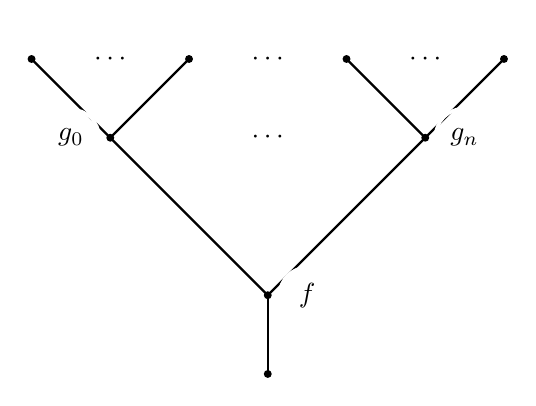
\begin{tikzpicture}[node distance={10mm}, thick, main/.style = {draw, circle, fill=black, inner sep=0pt, minimum width=2pt},
			letter/.style={circle,draw=white,very thick}] 
			
			\node[main] (1) {};
			\node[main] (p) at (2,0) {};
			\node[main] (p) at (4,0) {};
			\node[main] (p) at (6,0) {};
			\node[main] (p) at (1,-1) {};
			\node[main] (p) at (5,-1) {};
			\node[main] (p) at (3,-3) {};
			\node[main] (p) at (3,-4) {};
			
			\draw[-] (0,0) to (1,-1);
			\draw[-] (2,0) to (1,-1);
			\draw[-] (4,0) to (5,-1);
			\draw[-] (6,0) to (5,-1);
			\draw[-] (1,-1) to (3,-3);
			\draw[-] (5,-1) to (3,-3);
			\draw[-] (3,-3) to (3,-4);
			
			\node[letter] (p) at (1,0) {$\cdots$};
			\node[letter] (p) at (3,0) {$\cdots$};
			\node[letter] (p) at (5,0) {$\cdots$};
			\node[letter] (p) at (3,-1) {$\cdots$};
			\node[letter] (p) at (.5,-1) {$g_0$};
			\node[letter] (p) at (5.5,-1) {$g_n$};
			\node[letter] (p) at (3.5,-3) {$f$};
			
		\end{tikzpicture}
	\end{center}
	Además, para cualquier $a \in H_0$ tenemos una identidad $a \xrightarrow{\id_a} a$ en donde se satisfacen las siguientes propiedades:
	
	\begin{enumerate}
		\item Para cualquier $f:\vec{b} \to a$ en $H_1$, $f \cdot \id_a = f = \vec{\id}_{b_i} \cdot f$; y 
		\item Para cualesquiera $f: \vec{b} \to a$  y $g_i : \vec{c_i} \to b_i$ tenemos que: 
		
	\begin{center}
	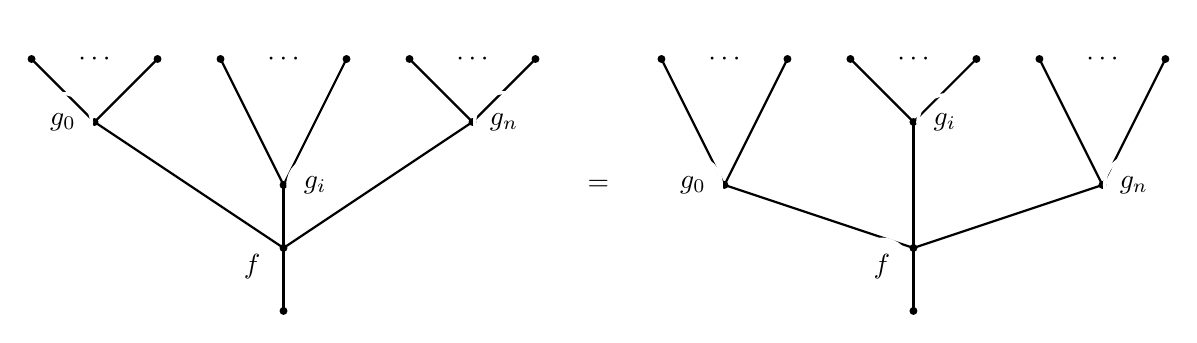
\begin{tikzpicture}[scale=0.8, node distance={10mm}, thick, main/.style = {draw, circle, fill=black, inner sep=0pt, minimum width=2pt},
		letter/.style={circle,draw=white,very thick}] 
		
		\node[main] (1) {};
		\node[main] (p) at (2,0) {};
		\node[main] (p) at (3,0) {};
		\node[main] (p) at (5,0) {};
		\node[main] (p) at (6,0) {};
		\node[main] (p) at (8,0) {};
		\node[main] (p) at (1,-1) {};
		\node[main] (p) at (7,-1) {};
		\node[main] (p) at (4,-2) {};
		\node[main] (p) at (4,-3) {};
		\node[main] (p) at (4,-4) {};
		
		\draw[-] (0,0) to (1,-1);
		\draw[-] (2,0) to (1,-1);
		\draw[-] (3,0) to (4,-2);
		\draw[-] (5,0) to (4,-2);
		\draw[-] (6,0) to (7,-1);
		\draw[-] (8,0) to (7,-1);
		\draw[-] (1,-1) to (4,-3);
		\draw[-] (7,-1) to (4,-3);
		\draw[-] (4,-3) to (4,-4);
		\draw[-] (4,-2) to (4,-3);
		
		\node[letter] (p) at (1,0) {$\cdots$};
		\node[letter] (p) at (4,0) {$\cdots$};
		\node[letter] (p) at (7,0) {$\cdots$};

		\node[letter] (p) at (.5,-1) {$g_0$};
		\node[letter] (p) at (4.5,-2) {$g_i$};
		\node[letter] (p) at (7.5,-1) {$g_n$};
		\node[letter] (p) at (3.5,-3.3) {$f$};
		
		\node[letter] (p) at (9,-2) {$=$};
		
		\node[main] (p) at (10,0) {};
		\node[main] (p) at (12,0) {};
		\node[main] (p) at (13,0) {};
		\node[main] (p) at (15,0) {};
		\node[main] (p) at (16,0) {};
		\node[main] (p) at (18,0) {};
		\node[main] (p) at (11,-2) {};
		\node[main] (p) at (14,-1) {};
		\node[main] (p) at (17,-2) {};
		\node[main] (p) at (14,-3) {};
		\node[main] (p) at (14,-4) {};
		
		\draw[-] (10,0) to (11,-2);
		\draw[-] (12,0) to (11,-2);
		\draw[-] (13,0) to (14,-1);
		\draw[-] (15,0) to (14,-1);
		\draw[-] (16,0) to (17,-2);
		\draw[-] (18,0) to (17,-2);
		\draw[-] (11,-2) to (14,-3);
		\draw[-] (17,-2) to (14,-3);
		\draw[-] (14,-1) to (14,-4);
		\draw[-] (14,-2) to (14,-3);
		
		\node[letter] (p) at (11,0) {$\cdots$};
		\node[letter] (p) at (14,0) {$\cdots$};
		\node[letter] (p) at (17,0) {$\cdots$};
		
		\node[letter] (p) at (10.5,-2) {$g_0$};
		\node[letter] (p) at (14.5,-1) {$g_i$};
		\node[letter] (p) at (17.5,-2) {$g_n$};
		\node[letter] (p) at (13.5,-3.3) {$f$};
		
	\end{tikzpicture}
	\end{center}
		
		
		
	\end{enumerate} 
Un \textbf{álgebra de signaturas de multicategorías} $F: \textbf{H} \to \textbf{N}$ es un morfismo de signatura de multicategorías compatible con la composición, es decir, cada que $\vec{c} \xrightarrow{\vec{g}} \vec{b} \xrightarrow{f} a$, $F(\vec{g} \cdot f) = F(\vec{g}) \cdot F(f)$ 
	Con estos morfismos, denotamos como $\textbf{MultiCat}$ a la categorías de multicategorías. 
\end{dfn}
Es importante resaltar que la propiedad $2$ nos indica intuitivamente que no importa el orden en que hagamos las composiciones, es decir, se respeta cierta noción de asociatividad. Aunque todavía no definimos formalmente el significado del cálculo en diagramas, lo analizaremos con precisión en el siguiente capítulo. \\ 
La signatura de multicategoría del ejemplo \ref{ej:RealSig} es propiamente un multicategoría con la composición dada de la manera natural. \\
De manera análoga al capítulo anterior, nuestra intención a continuación es definir una multicategoría libre. Antes, veamos la siguiente definición 

\begin{dfn}
	Sea $H$ una signatura de multicategoría. Sean $f:\vec{b} \to a$ y $g: \vec{c} \to b_i$ en $H_1$ con $i \in \{1, ..., n\}$ con $n$ es la aridad de $f$. \\
	Definimos la \textbf{composición parcial en la $i-$ésima entrada} como: 
	\[
		g \circ_i f = (\id_{b_1}\cdots g\cdots \id_{b_n})\cdot f 
	\]
	Gráficamente
	
	\begin{center}
		\begin{tikzpicture}[node distance={10mm}, thick, main/.style = {draw, circle, fill=black, inner sep=0pt, minimum width=2pt},
			letter/.style={circle,draw=white,very thick}] 
			
			\node[main] (1) {};
			\node[main] (p) at (2,0) {};
			\node[main] (p) at (4,0) {};
			\node[main] (p) at (6,0) {};
			
			\node[main] (p) at (0,-1) {};
			\node[main] (p) at (6,-1) {};
			\node[main] (p) at (3,-1) {};
			
			\node[main] (p) at (3,-2) {};
			
			\draw[-] (0,0) to (0,-1);
			\draw[-] (2,0) to (3,-1);
			\draw[-] (4,0) to (3,-1);
			\draw[-] (6,0) to (6,-1);
			\draw[-] (6,-1) to (3,-2);
			\draw[-] (0,-1) to (3,-2);
			\draw[-] (3,-1) to (3,-2);
			\draw[-] (3,-2) to (3,-3);
			
			\node[letter] (p) at (1,0) {$\cdots$};
			\node[letter] (p) at (3,0) {$\cdots$};
			\node[letter] (p) at (5,0) {$\cdots$};

			\node[letter] (p) at (-.5,-1) {$\id_{b_1}$};
			\node[letter] (p) at (6.5,-1) {$\id_{b_n}$};
			\node[letter] (p) at (3.5,-1.2) {$g$};
			\node[letter] (p) at (3.5,-2.3) {$f$};
			
		\end{tikzpicture}
	\end{center}
	
	
\end{dfn}
Una observación importante es que definimos la composición parcial a partir de la composición, pero también pudimos definirlo inversamente de la siguiente forma: 
\[
	[g_1\cdots g_n] \cdot f = g_{n}\circ_{n}(g_{n-1}\circ_{n-1}\dots \circ _2(g_1 \circ_1 f)...)
\]
Donde la propiedad $2$ de la composición para multicategorías nos garantiza que efectivamente la composición anterior coincide con la usual. \\
Con ello, ya estamos casi en condiciones de mostrar la construcción de una multicategoría libre, pero antes veamos una definición más.


\begin{dfn}
	Sea $H$ una signatura de multicategoría y sea $a \in H_0$, definimos recursivamente un \textbf{árbol con raíz $a$ de $H$}, como:
	\begin{itemize}
		\item Un nodo de la forma $w: \varepsilon \to a$ es un árbol (a los nodos de esta forma, les llamamos hojas);
		\item Un par $(f, (g_1, \dots , g_n))$ donde $f$ es un nodo de aridad $n$, $f:a_1a_2 \cdots a_n \to a$, y $g_1, \dots , g_n$ son nodos con codominios $a_1, \dots a_n$  es un arbol;
		\item Son todos.  
	\end{itemize}
\end{dfn}
Sea $H$ una signatura de multicategoría. $\textbf{Multi}(H)$ es la multicategoría cuyos objetos son exactamente los mismos que $H$ con los morfismos los árboles en $H$ y para cada objeto $a \in G_0$ tenemos la $\id_a$. La $i-$ésima composición parcial para morfismos $f, g$ en $\textbf{Multi}(H)$, $g \circ_i f$ está por reemplazar la $i-$ésima hoja de $f$ por una copia de $g$. \\
Decimos que dos árboles en $\textbf{Multi}(H)$ son iguales si puede ser obtenido uno a partir de otro mediante la aplicación consecutiva de las propiedades $1$ y $2$ para la composición en multicategorías. \\
De acuerdo presentado previamente, la composición parcial anterior induce correctamente la composición y, por lo tanto, $\textbf{Multi}(H)$ efectivamente es un multicategoría. 
Más aún, la construcción anterior es libre en virtud de la siguiente proposición.

\begin{prop}
	Sean $H$ una signatura de multicategorías, $\textbf{G}$ un multicategoría y $f:G_1 \to O_1$ una función que preserve la aridad de los nodos. Entonces existe un único morfismo de multicategorías $\varphi : \textbf{Multi}(H) \to \textbf{G}$ tal que el siguiente diagrama conmuta: 
	
	\[
	\begin{tikzcd}
		H \arrow{r}{\eta} \arrow{d}{i} & \textbf{G} \\
		\textbf{Multi}(H) \arrow{ur}{\varphi}
	\end{tikzcd}
	\] 
\end{prop} 

% Resta decir que $\textbf{Multi}: \textbf{MultiSig} \to \textbf{Multicat}$ es un funtor y, con ello, tenemos la siguiente proposición.
% \begin{prop}
% 	La construcción de una multicategoría libre es parte de la siguiente adjunción: 
% 	\begin{center}
% 	\begin{tikzpicture}[node distance={10mm}, thick, main/.style = {draw, circle, fill=black, inner sep=0pt, minimum width=2pt},
% 		letter/.style={circle,draw=white,very thick}] 
		
		
% 		\draw[->] (0,0.2) -- (1,0.2);
% 		\draw[->] (1,-0.2) -- (0,-0.2);

		
% 		\node[letter] (p) at (-1,0) {\textbf{MultiSig}};
% 		\node[letter] (p) at (2,0) {\textbf{MultiCat}};
% 		\node[letter] (p) at (.5,0.4) {\textbf{Multi}};
% 		\node[letter] (p) at (.5,-0.4) {\textbf{U}};

% 	\end{tikzpicture}
% 	\end{center}
% 	donde \textbf{U} es el funtor olvidadizo de una multigráfica a su signatura.

% \end{prop}

\section{Lenguajes libres de contexto}

Sea $G$ una signatura finita de multicategoría. Consideremos sus objetos como símbolos, los nodos como reglas de producción y los morfismos en \textbf{Multi}(G) como derivaciones, entonces obtenemos la noción de una gramática, más precisamente:

\begin{dfn}
	Un \textbf{gramática de multicategorías} es una signatura finita de multicategoría de la siguiente forma: 
	\[
		(B+V)^* \xleftarrow{\dom} G \xrightarrow[]{\cod} B
	\]
	donde $V$ es un vocabulario y $B$ es un conjunto de símbolos no terminales con un símbolo distinguido $s \in B$ y $G$ un conjunto de reglas de producciones. \\ El lenguaje generado por $G$ es: 
	\[
		\mathcal{L}(G) = \{ u \in V^*|\exists g: u \to s \in \textbf{Multi}(G) \}
	\]
\end{dfn}
Para comprender la definición anterior, consideremos los siguientes ejemplos. 

\begin{ej}
	El lenguaje de la lógica proposicional. Sea el conjunto de símbolos terminales vacío, el vocabulario $V=Var \cup \{ \wedge, \neg, (, ) \}$ donde $Var$ es el conjunto de letras proposicionales con las asignaciones:
	$$\text{para todo }p \in Var, \qquad p \to s$$
	y las reglas de producción 
	$$(s \wedge s) \to s \qquad \qquad \neg s \to s$$
	Con lo anterior, podemos obtener, por ejemplo, la siguiente derivación
	\begin{figure}[H]
		\includegraphics[scale=0.2]{diagrama/derivacion1.pdf}
		\centering
	\end{figure}
\end{ej}

\begin{ej}
	Consideremos el siguiente conjunto de símbolos $B=\{ n,v,a,c,p \}$ que corresponde a sustantivo, verbo, artículo, complemento y predicado; el vocabulario $V=\{ Naomi, come, un, taco \}$; las asignaciones 
	$$Naomi \to n \qquad come \to v \qquad un \to n \qquad taco \to n$$
	y las reglas de producción 
	$$(a, n) \to c \qquad (v,c) \to p \qquad (n,p) \to s$$
	Tenemos la siguiente derivación
	\begin{figure}[H]
		\includegraphics[scale=0.35]{diagrama/derivacion2.pdf}
		\centering
	\end{figure}
\end{ej}


Ahora, como anunciamos al inicio del capítulo, mostraremos la relación entre los lenguajes anteriores con la jerarquía de Chomsky. Para ello, veamos las siguientes definiciones y resultados.

\begin{dfn}
	
	Una gramática libre de contexto es una tupla $G=(V,B,P,s)$ donde $V$ es un vocabulario, $B$ es un conjunto de símbolos no terminales con un símbolo distinguido $s$ y $P$ es un conjunto de reglas de producción de la forma $A \to \alpha$ donde $A$ es un símbolo no terminal y $\alpha \in (V+B)^*$.\\
	Si $A \to \alpha$ es una regla de producción, para cualquier $\beta, \gamma \in (V+B)^*$ definimos la derivación 
	$\beta A \gamma \Rightarrow \beta \alpha \gamma$. 
	Consideramos $\Rightarrow ^*$ como la  cerradura transitiva de $\Rightarrow$. \\
    Definimos el lenguaje generado por $G$ como:
	
	$$ \mathcal{L}(G)= \{ w \in V^* | \exists s \Rightarrow w \} $$
	Decimos que un lenguaje $L$ es libre de contexto si existe una gramática $G$ libre de contexto tal que $L=L(G)$
\end{dfn}
Observemos que una oración en un lenguaje libre de contexto corresponde a una cadena en $V^*$ que puede ser derivada a partir de $s$ en $G$. \\
Ahora, la manera anterior de describir el lenguaje es eficiente para la generación de nuevas expresiones, sin embargo, puede no ser muy útil para el propósito de discriminar si una expresión dada pertenece, o no, al lenguaje. Con ese propósito surgen los árboles de derivación. 
\begin{dfn}
	Sea $G=(V,B,P,s)$ una gramática libre de contexto. \\
	Un árbol es un árbol de derivación para $G$ si:
	\begin{itemize}
		\item Cada vértice está etiquetado con un símbolo de $V \cup B \cup \{ \varepsilon \}$; 
		\item la raíz del árbol es $s$; 
		\item si un vértice interior está etiquetado con A, entonces $A \in B$, es decir, no es un símbolo terminal;
		\item si un vértice $A$ tiene $n$ hijos, $A_1, \dots, A_n$, entonces:
		$$A \to A_1A_2 \cdots A_n$$
		es una regla de producción en $P$; y
		\item si un vértice está etiquetado con $\epsilon$, entonces es un hoja y, además, es el único hijo de su padre.
	\end{itemize}
\end{dfn}
Notemos que el diagrama del ejemplo uno corresponde a un árbol de derivación en la gramática $A \to \neg A | A \land A | A \lor A | A \to A | A \leftrightarrow A|a_0|a_1|a_2 $.\\ 
Con esto, podemos enunciar la siguiente proposición cuya prueba podemos consultar en \cite{hopcroft01}. \\
\begin{prop}
	Sea $G=(V,B,P,s)$ una gramática libre de contexto. Entonces $s \Rightarrow ^* w$ si y solo si existe un árbol de derivación para $G$ que produce a $w$. 
\end{prop}

Dada la definición de morfismos en una multicategoría libre, es inmediato notar que los morfismos de la forma $f:u \to s$ con $u \in V^*$ en una gramática de multicategoría son árboles de derivaciones y viceversa. Así, tenemos el siguiente teorema con el cual terminamos el presente capítulo.  
\begin{thm}
	Sea $G$ una signatura de multicategoría y $G'$ una gramática libre de contexto, entonces\\
	1. $L(G)$ es un lenguaje libre de contexto.\\
	2. Existe una signatura de multigráfica que genera a $L(G')$. 
\end{thm}

\end{document}